\documentclass[8pt,t]{beamer}

\newcommand{\rb}[1]{\left( #1 \right)}
\renewcommand{\sb}[1]{\left[ #1 \right]}
\newcommand{\cb}[1]{\left\{ #1 \right\}}
\newcommand{\ab}[1]{\left\langle #1 \right\rangle}

\newtheorem{algorithm}{Algorithm}
\newtheorem{proposition}{Proposition}

\newcommand{\threebyone}[3]{
  \begin{pmatrix}
    #1 \\
    #2 \\
    #3
  \end{pmatrix}
}

\newcommand{\threebythree}[9]{
  \begin{pmatrix}
    #1 & #2 & #3 \\
    #4 & #5 & #6 \\
    #7 & #8 & #9
  \end{pmatrix}
}

\newcommand{\function}[5][]{
  \ifx &#1&
    \begin{array}{rcl}
      #2 & \to     & #3 \\
      #4 & \mapsto & #5
    \end{array}
  \else
    \begin{array}{crcl}
      #1 : & #2 & \to     & #3 \\
           & #4 & \mapsto & #5
    \end{array}
  \fi
}

\newcommand{\C}{\mathbb{C}}
\newcommand{\R}{\mathbb{R}}
\newcommand{\Q}{\mathbb{Q}}
\newcommand{\Z}{\mathbb{Z}}
\newcommand{\N}{\mathbb{N}}

\newcommand{\A}{\mathbb{A}}
\renewcommand{\P}{\mathbb{P}}

\newcommand{\OO}{\mathcal{O}}

\title{An unusual cubic representation problem}
\author{David Kurniadi Angdinata}
\date{Wednesday, 16 January 2019}

\begin{document}

\begin{frame}
\maketitle
\end{frame}

\begin{frame}{An unusual cubic representation problem}
\begin{center}
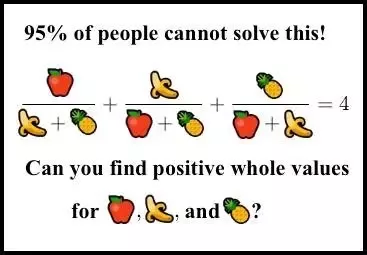
\includegraphics[width=0.7\textwidth]{img/positive_whole_values.png}
\end{center}
\pause
\begin{align*}
\textsc{apple} & = \text{\tiny 154476802108746166441951315019919837485664325669565431700026634898253202035277999} \\
\textsc{banana} & = \text{\tiny 36875131794129999827197811565225474825492979968971970996283137471637224634055579} \\
\textsc{pineapple} & = \text{\tiny 4373612677928697257861252602371390152816537558161613618621437993378423467772036}
\end{align*}
\end{frame}

\begin{frame}{A trivial cubic representation problem}
\begin{center}
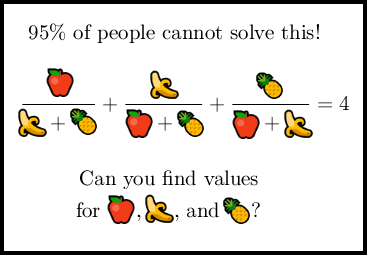
\includegraphics[width=0.7\textwidth]{img/values.png}
\end{center}
\pause
$$
\begin{array}{lllll}
\C, \R & : & \rb{a, b, c} & = & \rb{2 + \sqrt{3}, 1, 0} \\
\pause
& & \\
\Q, \Z & : & \rb{a, b, c} & = & \rb{11, 4, -1} \\
\pause
& & & = & \rb{-11, -4, 1} \\
\pause
& & & = & \rb{1, -4, -11} \\
& & & = & \dots
\end{array}
$$
\end{frame}

\begin{frame}{A less unusual cubic representation problem}
\framebox[\linewidth]{$ \dfrac{a}{b + c} + \dfrac{b}{a + c} + \dfrac{c}{a + b} = 4, \qquad a, b, c \in \Z. $} \vspace{0.1cm} \\
\begin{itemize}
\item Require $ a, b, c > 0 $.
\end{itemize}
\pause
Clear denominators:
\only<3>{$$ \rb{\dfrac{a}{b + c} + \dfrac{b}{a + c} + \dfrac{c}{a + b}}\rb{a + b}\rb{a + c}\rb{b + c} $$
$$ = 4\rb{a + b}\rb{a + c}\rb{b + c}. $$}
\only<4>{$$ a\rb{a + b}\rb{a + c} + b\rb{a + b}\rb{b + c} + c\rb{a + c}\rb{b + c} $$
$$ = 4\rb{a + b}\rb{b + c}\rb{a + c}. $$}
\only<5>{$$ a^3 + a^2c + a^2b + abc + ab^2 + abc + b^3 + b^2c + abc + ac^2 + bc^2 + c^3 $$
$$ = 4a^2b + 4abc + 4a^2c + 4ac^2 + 4ab^2 + 4b^2c + 4abc + 4bc^2. $$}
\only<6->{$$ a^3 + b^3 + c^3 - 5abc - 3\rb{a^2b + ab^2 + a^2c + ac^2 + b^2c + bc^2} = 0. $$}
\only<7->{\textbf{Trivial} solutions:
$$
\begin{array}{lll}
\rb{a, b, c} & = & \rb{11, 4, -1} \\
& = & \rb{-11, -4, 1} \\
& = & \rb{1, -4, -11} \\
& = & \dots
\end{array}
$$}
\only<8->{\textbf{Invalid} solutions:
$$
\begin{array}{lll}
\rb{a, b, c} & = & \rb{1, -1, 0} \\
& = & \rb{-1, 1, 0} \\
& = & \rb{-1, 1, -1} \\
& = & \dots
\end{array}
$$}
\only<9->{\begin{itemize}
\item Require $ a + b, a + c, b + c > 0 $.
\end{itemize}}
\end{frame}

\begin{frame}{Dimensionality of solution space}
\framebox[\linewidth]{$ a^3 + b^3 + c^3 - 5abc - 3\rb{a^2b + ab^2 + a^2c + ac^2 + b^2c + bc^2} = 0, \qquad a, b, c \in \Z $} \vspace{0.1cm} \\
\begin{definition}
A polynomial is \textbf{homogeneous} if all of its monomials have the same total degree.
\end{definition}
\pause
\begin{proposition}
If $ \rb{a_0, b_0, c_0} $ is a solution in $ \Z $, then $ \rb{\lambda a_0, \lambda b_0, \lambda c_0} $ is a solution in $ \Q $ for any $ \lambda \in \Q^* $.
\end{proposition}
\pause
Define the equivalence relation $ \sim $ by
$$ \rb{a_0, b_0, c_0} \sim \rb{a_0', b_0', c_0'} \qquad \iff \qquad \rb{a_0, b_0, c_0} = \rb{\lambda a_0', \lambda b_0', \lambda c_0'} \ \text{for some} \ \lambda \in \Q^*. $$
Write the equivalence class as $ \sb{a_0, b_0, c_0} $.
\pause
\begin{itemize}
\item Modulo $ \sim $, the space of solutions to the equation is only two-dimensional.
\end{itemize}
\pause
\begin{proposition}
If $ c \ne 0 $, the equation is equivalent to
$$ a^3 + b^3 + 1 - 5ab - 3\rb{a^2b + ab^2 + a^2 + a + b^2 + b} = 0, \qquad a, b \in \Q. $$
\end{proposition}
\pause
\begin{itemize}
\item Modulo $ \sim $, the equation is cubic of two variables.
\end{itemize}
\end{frame}

\begin{frame}{Elliptic curves: informally}
\begin{center}
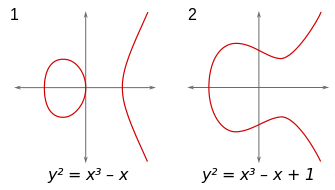
\includegraphics[width=0.5\textwidth]{img/ECClines-3.png}
\end{center}
An \textit{elliptic curve} is the space of solutions to a cubic equation
$$ y^2 = x^3 + Ax + B, $$
where $ A $ and $ B $ are in some field such that $ 4A^3 + 27B^2 \ne 0 $.
\begin{itemize}
\item Simplest non-trivial structures in algebraic geometry.
\item Topic of the \textit{Birch and Swinnerton-Dyer conjecture}.
\item Tool in Wiles' proof of \textit{Fermat's last theorem}.
\item Methods for primality testing and integer factorisation.
\item Applications in \textit{elliptic curve cryptography}.
\end{itemize}
\end{frame}

\begin{frame}{Elliptic curves: formally}
\begin{definition}
An \textbf{elliptic curve} over a \textit{perfect field} $ K $ is a \textit{smooth projective plane algebraic curve} $ E $ of \textit{genus one} with a \textit{flex $ K $-rational base point} $ \OO_E $.
\begin{itemize}
\item<2-> \textit{algebraic curve}: space of solutions to equation
\item<3-> \textit{plane}: two variables
\item<4-> \textit{projective}: consider equivalence classes of solutions
\item<5-> \textit{smooth}: no kinks
\item<6-> \textit{genus one}: degree three
\item<7-> \textit{$ K $-rational base point}: $ K $ coordinates
\item<8-> \textit{flex}: tangent has intersection multiplicity three
\item<9-> \textit{perfect field}: every algebraic extension is separable
\end{itemize}
\end{definition}
\only<10>{\begin{theorem}
An elliptic curve over $ \Q $ is of the form
$$ E = \cb{\rb{x, y} \in \Q^2 \mid y^2 = x^3 + Ax + B} \cup \cb{\OO}, $$
for some $ A, B \in \Q $ such that $ 4A^3 + 27B^2 \ne 0 $, where $ \OO = \sb{0, 1, 0} $.
\end{theorem}}
\end{frame}

\begin{frame}{Weierstrass representations}
\framebox[\linewidth]{$ a^3 + b^3 + c^3 - 5abc - 3\rb{a^2b + ab^2 + a^2c + ac^2 + b^2c + bc^2} = 0, \qquad a, b, c \in \Z $} \vspace{0.1cm} \\
\begin{proposition}
The curve given by the equation is isomorphic to the following elliptic curves.
\begin{itemize}
\item<2-> $ \cb{\rb{x, y} \in \Q^2 \mid 6y^2 + 6xy + 6y = -91x^3 + 141x^2 + 15x - 1} \cup \cb{\OO} $.
\item<3-> $ \cb{\rb{x, y} \in \Q^2 \mid y^2 + xy - \tfrac{91}{6}y = x^3 + \tfrac{47}{2}x^2 - \tfrac{455}{12}x - \tfrac{8281}{216}} \cup \cb{\OO} $.
\item<4-> $ \cb{\rb{x, y} \in \Q^2 \mid y^2 + xy + y = x^3 - 234x + 1352} \cup \cb{\OO} $.
\item<5-> $ \cb{\rb{x, y} \in \Q^2 \mid y^2 = x^3 + \tfrac{1}{4}x^2 - \tfrac{467}{2}x + \tfrac{5409}{4}} \cup \cb{\OO} $.
\item<6-> $ \cb{\rb{x, y} \in \Q^2 \mid y^2 = x^3 + 109x^2 + 224x} \cup \cb{\OO} $.
\item<7-> $ \cb{\rb{x, y} \in \Q^2 \mid y^2 = x^3 - \tfrac{11209}{48}x + \tfrac{1185157}{864}} \cup \cb{\OO} $.
\item<8-> $ \cb{\rb{x, y} \in \Q^2 \mid y^2 = x^3 - 302643x + 63998478} \cup \cb{\OO} $.
\end{itemize}
\end{proposition}
\only<9->{Let $ A = -302643 $ and $ B = 63998478 $.}
\only<10>{Overall invertible transformations:
$$
\begin{cases}
a = \tfrac{1}{72}x + \tfrac{1}{216}y - \tfrac{277}{24} \\
b = \tfrac{1}{72}x - \tfrac{1}{216}y - \tfrac{277}{24} \\
c = \tfrac{1}{6}x - \tfrac{95}{2}
\end{cases}
\qquad
\begin{cases}
x = \dfrac{1710a + 1710b - 831c}{6a + 6b - c} \\
y = \dfrac{-9828a + 9828b}{6a + 6b - c}
\end{cases}
$$}
\end{frame}

\begin{frame}{A group law}
\framebox[\linewidth]{$ E = \cb{\rb{x, y} \in \Q^2 \mid y^2 = x^3 + Ax + B} \cup \cb{\OO} $} \vspace{0.1cm} \\
\begin{theorem}
$ E $ is an abelian group $ \rb{E, +} $.
\begin{itemize}
\item<2-> The identity point is $ \OO \in E $.
\item<3-> The inverse of a point is obtained by reflecting the point about the $ x $-axis.
$$ -\rb{x, y} = \rb{x, -y}. $$
\item<4-> The sum of two points is obtained by inverting the third point of intersection between the curve and the line joining the two points.
$$ P + Q =
\begin{cases}
S & P = \rb{x, y}, \ Q = \rb{x', y'}, \ x \ne x' \\
R & P = Q = \rb{x, y}, \ y \ne 0 \\
P & Q = \OO \\
\OO & P = Q = \rb{x, 0}
\end{cases},
$$
$$ S = \rb{\tfrac{\rb{A + xx'}\rb{x + x'} + 2\rb{B - yy'}}{\rb{x - x'}^2}, \tfrac{\rb{Ay' - x'^2y}\rb{3x + x'} + \rb{x^2y' - Ay}\rb{x + 3x'} - 4B\rb{y - y'}}{\rb{x - x'}^3}}, $$
$$ R = \rb{\tfrac{x^4 - 2Ax^2 - 8Bx + A^2}{4y^2}, \tfrac{x^6 + 5Ax^4 + 20Bx^3 - 5A^2x^2 - 4ABx - A^3 - 8B^2}{8y^3}}. $$
\end{itemize}
\end{theorem}
\end{frame}

\begin{frame}{Proof of the group law}
\framebox[\linewidth]{$ E = \cb{\rb{x, y} \in \Q^2 \mid y^2 = x^3 + Ax + B} \cup \cb{\OO} $} \vspace{0.1cm} \\
\begin{theorem}
$ E $ is an abelian group $ \rb{E, +} $.
\end{theorem}
\pause
\begin{lemma}[B\'ezout's theorem]
Let $ C $ and $ D $ be projective algebraic curves over an algebraically closed field $ \overline{K} $. Then $ C $ and $ D $ intersect at exactly $ \deg C\deg D $ points counted with intersection multiplicity.
\end{lemma}
\pause
\begin{lemma}[Cayley-Bacharach theorem]
Let $ C, D, E $ be projective algebraic cubic curves over an algebraically closed field $ \overline{K} $ such that
$$ C \cap E = \cb{P_1, \dots, P_8, Q}, \qquad D \cap E = \cb{P_1, \dots, P_8, R}, $$
counted with intersection multiplicity. Then $ Q = R $.
\end{lemma}
\pause
\begin{itemize}
\item<4-> Well-definition of addition in $ K $ holds by explicit equations.
\item<5-> Commutativity of addition holds by symmetry.
\item<6-> Associativity of addition holds by intimidation.
\end{itemize}
\end{frame}

\begin{frame}{Procedure}
\begin{algorithm}
Generate new solutions from old solutions.
\begin{itemize}
\item<2-> Choose an initial solution for
$$ a^3 + b^3 + c^3 - 5abc - 3\rb{a^2b + ab^2 + a^2c + ac^2 + b^2c + bc^2} = 0, \qquad a, b, c \in \Z. $$
\item<3-> Apply the change of variables:
$$
\begin{cases}
x = \dfrac{1710a + 1710b - 831c}{6a + 6b - c} \\
y = \dfrac{-9828a + 9828b}{6a + 6b - c}
\end{cases}.
$$
\item<4-> Compute multiples of point in
$$ y^2 = x^3 + Ax + B, \qquad \rb{x, y} \in \Q^2. $$
\item<5-> Apply the change of variables:
$$
\begin{cases}
a = \tfrac{1}{72}x + \tfrac{1}{216}y - \tfrac{277}{24} \\
b = \tfrac{1}{72}x - \tfrac{1}{216}y - \tfrac{277}{24} \\
c = \tfrac{1}{6}x - \tfrac{95}{2}
\end{cases}.
$$
\item<6-> Terminate or repeat.
\end{itemize}
\end{algorithm}
\end{frame}

\begin{frame}{Computation: failure}
Choose an invalid solution:
$$ \rb{a, b, c} = \rb{-1, 1, -1}. $$
\pause
\begin{itemize}
\item Apply the change of variables:
$$ \rb{x, y} = \rb{831, 19656}. $$
\end{itemize}
\pause
Compute multiples of point:
\begin{itemize}
\item<4-> $ 1\rb{x, y} = \rb{831, 19656} $.
\item<5-> $ 2\rb{x, y} = \rb{363, 1404} $.
\item<6-> $ 3\rb{x, y} = \rb{327, 0} $.
\item<7-> $ 4\rb{x, y} = \rb{363, -1404} $.
\item<8-> $ 5\rb{x, y} = \rb{831, -19656} $.
\item<9-> $ 6\rb{x, y} = \OO $.
\end{itemize}
\only<10->{This is a cyclic subgroup of order six.}
\end{frame}

\begin{frame}{Computation: success}
Choose a trivial solution:
$$ \rb{a, b, c} = \rb{11, 4, -1}. $$
\pause
\begin{itemize}
\item Apply the change of variables:
$$ \rb{x, y} = \rb{291, -756}. $$
\end{itemize}
\pause
Compute multiples of point:
\begin{itemize}
\item<4-> $ 1\rb{x, y} = \rb{291, -756} $.
\item<5-> $ 2\rb{x, y} = \rb{\tfrac{22107}{49}, -\tfrac{1506492}{343}} $.
\begin{itemize}
\item<6-> Apply the change of variables:
$$ \rb{a, b, c} = \rb{-8784, 5165, 9499}. $$
\end{itemize}
\item<7-> $ 3\rb{x, y} = \rb{-\tfrac{2694138}{11881}, -\tfrac{14243306490}{1295029}} $.
\begin{itemize}
\item<8-> Apply the change of variables:
$$ \rb{a, b, c} = \rb{679733219, -375326521, 883659076}. $$
\end{itemize}
\item<9-> $ 9\rb{x, y} = (\tfrac{3823387580080160076063605209061052603963389916327719142}{13514400292716288512070907945002943352692578000406921}, $
$$ -\tfrac{1587622549247318249299172296638373895912313166958011719500537215259315694916502670}{1571068668597978434556364707291896268838086945430031322196754390420280407346469}). $$
\begin{itemize}
\item<10-> Apply the change of variables:
$$ \rb{a, b, c} = \rb{\textsc{apple}, \textsc{banana}, \textsc{pineapple}}. $$
\end{itemize}
\end{itemize}
\end{frame}

\begin{frame}{Further facts}
The general equation is
$$ \dfrac{a}{b + c} + \dfrac{b}{a + c} + \dfrac{c}{a + b} = N, \qquad a, b, c \in \N^*, \qquad N \in \Z. $$
\begin{itemize}
\item<2-> The curve is
$$ E \cong \Z^r \oplus
\begin{cases}
\Z / 2\Z \oplus \Z / 6\Z & N = 2 \\
\Z / 6\Z & \text{otherwise}
\end{cases},
\qquad r \in \N^*. $$
\begin{itemize}
\item<3-> The curve for $ N = 4 $ has $ r = 1 $.
\end{itemize}
\item<4-> The smallest solution for $ N = 4 $ is $ \rb{a, b, c} = \rb{\textsc{apple}, \textsc{banana}, \textsc{pineapple}} $.
\begin{itemize}
\item<5-> Proof by heights.
\end{itemize}
\item<6-> The smallest solution for $ N = 178 $ has four hundred million digits.
\begin{itemize}
\item<7-> More than the twenty volume second edition of the Oxford English Dictionary.
\end{itemize}
\item<8-> There are no solutions for $ N $ is odd.
\begin{itemize}
\item<9-> Proof by congruences.
\end{itemize}
\item<10-> There may also be no solutions if $ N $ is even.
\begin{itemize}
\item<11-> There are infinitely many even $ N $ with solutions.
\end{itemize}
\end{itemize}
\end{frame}

\begin{frame}{Further references}
A Amit's 2017 Quora answer on \textit{How do you find the positive integer solutions to}
$$ \dfrac{x}{y + z} + \dfrac{y}{z + x} + \dfrac{z}{x + y} = 4? $$ \vspace{0.4cm} \\
A Bremner and A Macleod's 2014 paper on \textit{An unusual cubic representation problem} \vspace{1cm} \\
J Silverman's 1986 book on \textit{The arithmetic of elliptic curves} \vspace{1cm} \\
R Hartshorne's 1977 book on \textit{Algebraic geometry} \vspace{1cm} \\
N Duif's 2011 implementation on \textit{Transforming a general cubic elliptic curve equation to Weierstrass form} \vspace{0.7cm} \\
M Laska's 1982 paper on \emph{An algorithm for finding a minimal weierstrass equation for an elliptic curve}
\end{frame}

\end{document}